\documentclass[a4paper,12pt]{report}
\def\magyarOptions{defaults=hu-min}

\usepackage[magyar]{babel}
\usepackage{t1enc}
\usepackage{indentfirst}
\usepackage[utf8]{inputenc}
\usepackage{url}
\usepackage{times}
\usepackage{subfigure}
\usepackage{amsmath}
\usepackage{amssymb}
\usepackage{amsthm}
\usepackage{verbatim}
\usepackage{fancyhdr}
\usepackage{graphicx}
\usepackage{psfrag}
\usepackage{setspace}
\usepackage[numbers]{natbib}
\usepackage{color}
\usepackage{xcolor}
\usepackage{listings}
\usepackage{todonotes}
\usepackage{rotating}

\bibliographystyle{abbrvnat}

\hoffset -0.85in
\voffset -1.5in
\oddsidemargin 30mm
\evensidemargin 20mm
\textwidth 150mm
\topmargin 30mm
\textheight 237mm
\onehalfspacing

\definecolor{codegreen}{rgb}{0,0.6,0}
\definecolor{codegray}{rgb}{0.5,0.5,0.5}
\definecolor{codepurple}{rgb}{0.58,0,0.82}
\definecolor{backcolour}{rgb}{0.95,0.95,0.92}
 
\lstdefinestyle{mystyle}{
    backgroundcolor=\color{backcolour},   
    commentstyle=\color{codegreen},
    keywordstyle=\color{magenta},
    numberstyle=\tiny\color{codegray},
    stringstyle=\color{codepurple},
    basicstyle=\footnotesize,
    breakatwhitespace=false,         
    breaklines=true,                 
    captionpos=b,                    
    keepspaces=true,                 
    numbers=left,                    
    numbersep=5pt,                  
    showspaces=false,                
    showstringspaces=false,
    showtabs=false,                  
    tabsize=2
}
\renewcommand{\lstlistingname}{Forráskód}
\lstset{style=mystyle}

%%%%%%%%%%%%%%%%%%%%%%%%%%%%%%%%%%%%%%%%%%%%%%%%%%%%%%

\begin{document}

\begin{singlespace}

\fancypagestyle{plain}{
\fancyhf{}
\fancyfoot[R]{\thepage}
\renewcommand{\headrulewidth}{0pt}
}

\pagestyle{fancy}
\fancyhf{}
\fancyhead[R]{Tömegérzékeléses adatgyűjtés okos közlekedési alkalmazásokhoz}
\fancyfoot[R]{\thepage}

\thispagestyle{empty}

\begin{center}
\vspace*{1cm}
{\Large\bf Debreceni Egyetem}
\vspace{0.2cm}

{\Large\bf Informatikai Kar}
\vspace{0.2cm}

{Információ Technológia Tanszék}
\vspace*{2.8cm}

{\LARGE\bf Tömegérzékeléses adatgyűjtés okos közlekedési alkalmazásokhoz}
\vspace*{7cm}


{\large
\begin{tabular}{c@{\hspace{3cm}}c}
\emph{Témavezető:}      &       \emph{Készítette:}\\
\bf{dr. Bátfai Norbert} &       \bf{Besenczi Renátó}\\
egyetemi adjunktus      &        mérnökinformatikus hallgató\\
\end{tabular}
}

\vspace*{1cm}
\end{center}

\vspace{45mm}
\begin{center}
{\Large
Debrecen
\\
\vspace{2mm}
2015
}
\end{center}

\tableofcontents

\end{singlespace}
%%%%%%%%%%%%%%%%%%%%%%%%%%%%%%%%%%%%%%%%%%%%%%%%%%%%%%%%%%%%%%%%%%%%%%%%%%%%%%%%%%%%%%%%%%%%%%%%%%%%%%%%%%%%%%%%%%%%%%%%%%%

\chapter{Bevezetés és célkitűzések}

2050-re a világ lakosságának 70\%-a várhatóan városokban fog élni \cite{unpopulation}. Ez a nagy mértékű urbanizáció új kihívások elé állítja a városi infrastruktúrát. Hogyan kezelhető egy ekkora méretű népesség? Milyen szolgáltatásokat nyújtson a városi adminisztráció annak érdekében, hogy élhető maradjon a város? Többek között ezekre a kérdésekre ad választ a Smart City kutatási terület, melynek megoldásai az utóbbi években kezdenek egyre inkább a mindennapok részévé válni. Kiemelten fontos problémakör lehet (és részben már most is az) a városi közlekedés. Egyre többen használják a városi infrastruktúrát, így a városi úthálózatot is. Milyen alkalmazást tud nyújtani a városi menedzsment, hogy a lakosok optimális módon tudjanak közlekedni? Erre a kérdésre adhat választ az okos közlekedés menedzsment (Smart traffic management).

A tömegérzékelés (crowd-sensing és crowd-sourcing) egy olyan eszközkészlet, mellyel bizonyos méréseket végezhetünk a lakosságra nézve, illetve a lakosság bevonásával. Ezek a mérések kiemelt szerepet játszanak az egyes döntési folyamatok során, valamint bemeneti adatként szolgálhatnak különféle szcenárióelemzésekhez, vagy akár konkrét szimulációkhoz is (ahogyan azt a dolgozat következő fejezeteiben is látni fogjuk). Egészen pontosan fogalmazva: a városi lakosságról íly módon szerezhetünk konkrét információkat, elemezhetjük szokásaikat egy számunkra érdekes kontextusban (példaul: hogyan közlekednek a városon belül). Habár a mérés az egyén szintjén történik, a lényeges információ nem ezen a szinten jelentkezik, így az elemzést egy aggregált, absztrakt szinten, a tömeg szintjén végezzük (individual level processing, crowd level analysis).

A korábbi években igen sok fejlődés tapasztalható az autógyártásban, elsősorban az autonóm autók kapcsán. Egyre több autógyártó és techóriás fejleszt robotautót, mint például a területen úttörő Google (a fejlesztői prototípus a \ref{googleauto} képen látható) vagy a Volkswagen cégcsoport, de a Tesla elektromos autó gyártó termékei is egyre inkább önjáróak. Ezek a trendek folyamatosan gyorsulni látszanak. A 2000-es és 2010-es éveket főként az autókba épített, vezetőt segítő elektronikai eszközök uralták (úgymint a gyalogosfigyelő rendszerek, sávelhagyásra figyelmeztető rendszerek, stb.), a 2020-as éveket várhatóan az autonóm autók széles körű elterjedése fogja meghatározni. Ezek mellett a tisztán elektromos hajtású, valamint 2015-től a piacon is elérhető hidrogénhajtású autók is egyre szélesebb körben elérhetőek. Világosan látható, hogy az autóipar paradigmaváltás előtt áll. A vezetői élmény jelentősége és a fosszilis energiaforrásokon alapú hajtásláncok folyamatosan visszaszorulnak, helyettük a hosszú távon is fenntartható, környezetbarát, az utazást, mint pihentető, emberbarát eseményt vízionáló megoldások kerülnek a figyelem középpontjába.

\begin{figure}[h]
\centerline{
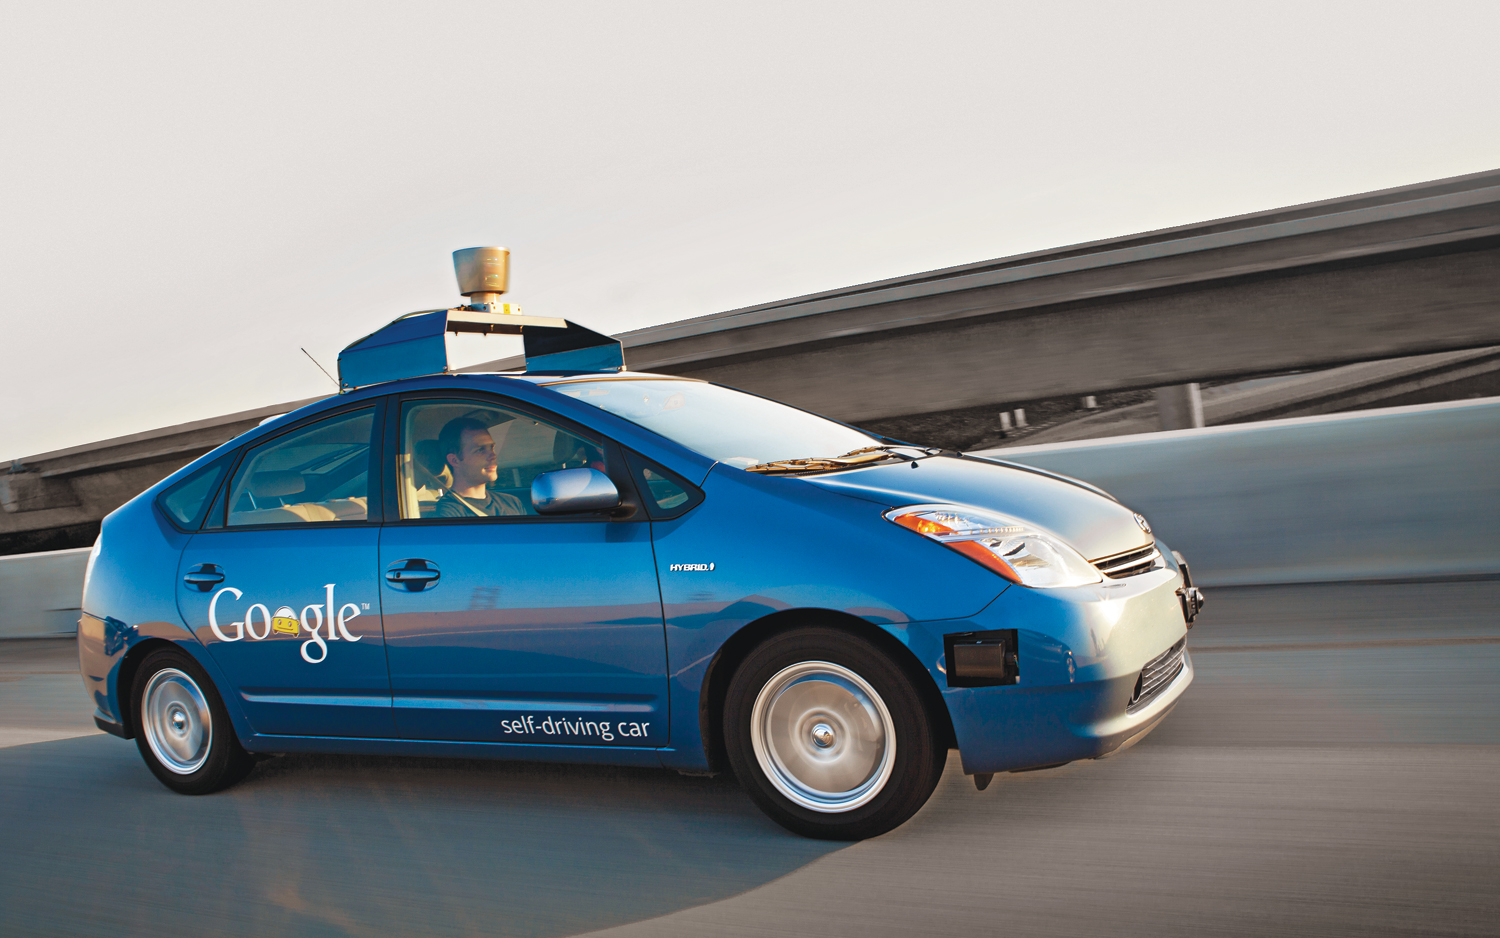
\includegraphics[width=6in]{img/googleauto}}
\caption{A Google által fejlesztett robotautó fejlesztői prototípusa.}
\label{googleauto}
\end{figure}

A két terület találkozási pontja egyértelmű: egy teljesen ésszerű elképzelés, hogy a már most is fejlett elektronikával szerelt autóknak a város adjon útvonalat. Ugyanis a városnak rendelkezésére állhat minden olyan információ, amellyel az utazás optimálissá, gazdaságosabbá, gyorsabbá tehető. Ilyen információk az útlezárások, felújítások, elterelések, vagy például ritka események, balesetek. 

Jelen dolgozat egy olyan tömegérzékeléses eszköz kiépítésének technikai és elméleti oldalát mutatja be, mellyel egy városi adminisztráció folyamatosan képes monitorozni a forgalmat. Az eszköz hardware illetve software komponensekből épül fel, és képes valós időben adatot gyűjteni a körülötte lévő forgalmi helyzetről, azt továbbítani egy szerveralkalmazás felé. A prototípussal egy próbamérést végeztünk, az adatokat elemeztük, aggregáltuk, majd egy forgalomszimulációra alkalmas rendszerben teszteltük, így megfigyelhetővé vált a forgalmi helyzet változása a kiinduló adatokhoz képest. Ennek az eszköznek a segítségével, valamint a későbbiekben leírt forgalomszimulációs rendszer segítségével képesek vagyunk pontosabb, a forgalmi helyzetet is figyelembe vevő útvonalat tervezni a forgalomban résztvevő egységeknek.

A dolgozat az alábbiak szerint épül fel: a következő fejezetben egy kitekintést adunk a Smart City kutatási-fejlesztési területre, majd röviden bemutatjuk a Robocar World Championship (vagy röviden OOCWC) rendszer felépítését és működését. A \ref{rttachapter}. fejezetben részletesen bemutatjuk a fejlesztett adatgyűjtő rendszert, a működésével szemben támasztott követelményeket és a tervezést (\ref{tervezes}. rész), a hardware (\ref{rttahw}. rész) és a software (\ref{rttasw}. rész) működését, valamint a felhasznált fejlesztőeszközöket (\ref{dev}. rész). A \ref{cstschapter}. fejezetben bemutatjuk a mért adatokon alapuló szimulációt. A \ref{results}. fejezetben összegezzük az eredményeinket, valamint adunk egy rövid konklúziót.

\chapter{Kapcsolódó kutatások}

A Okos Város kutatási, fejlesztési terület jelentős szerepet fog játszani az következő évtizedekben. Előrejelzések szerint 2023-ig több mint 170 milliárd dollár beruházás fog megvalósulni világszerte \cite{navigant}. A különböző informatikai megoldások egyre nagyobb számban vannak jelen a hétköznapokban már napjainkban is, mint például a VITAL \cite{vital}, a FI\-Ware \cite{fiware} vagy az iCity \cite{icity}. Ezen felül egyre több kezdeményezés tesz kísérletet arra, hogy a városi lakosság hétköznapjait okosabbá és biztonságosabbá tegye (\cite{smartsantander}, \cite{futureglasgow}, \cite{myneighbourhood}). Emellett sok tanulmány foglalkozik a smart city fogalomkörével, illetve hogyan mérhető egy város ``smartsága'' (\cite{yamauchi2014development}, \cite{neirotti2014current}, \cite{de2014smart}, \cite{carli2013measuring}). A \cite{giffinger2007smart} tanulmány egy sorrendet is felállított az európai városokról ``smartság'' tekintetében. A vészhelyzetek kezelése is kiemelt szerepet kap (például \cite{du2012research}). A témánkhoz kapcsolódóan megemlíthető, hogy a \cite{mohan2008nericell} szerzői egy mobiltelefon alapú, automatikus forgalommérő rendszert fejlesztettek.

Látható, hogy a Smart City kutatási, fejlesztési terület lassan iparággá növi ki magát, mindenképpen komoly jövő előtt áll.

Az adatgyűjtés fontos alapokat szolgáltat az okos város alkalmazásoknak. Legyen szó egy döntési folyamatról vagy csupán egyszerű monitorozásról, az adatgyűjtő rendszerek jelentős részét képezik bármely okos szolgáltatásnak. Az adatgyűjtés módja szerint két fő kategóriát különíthetünk el.

\begin{itemize}
\item Crowd-sourcing -- ahol a felhasználó aktív részvétele szükséges
\item Crowd-sensing -- ahol a felhasználó aktív részvétele nem szükséges
\end{itemize}

Tehát a két módszer a felhasználó részvétele alapján különíthető el. A crowd-sourcing esetében a felhasználó megfigyel valamilyen eseményt, és valamilyen eszköz használatával küld adatot (participatory sensing). Ilyen adatgyűjtő rendszerek találhatóak a \cite{szabo2013framework} közleményben, illetve egy rendszer implementációjának részletes leírása a \cite{besenczi2013kozossegi} szakdolgozatban. Ezzel szemben a crowd-sensing nem igényel emberi beavatkozást, a rendszer autonóm módon működik.

A rendszer által gyűjtött adatok a Robocar World Championship (vagy röviden OOCWC) rendszer bemeteként szolgáltak. A OOCWC rendszer célja, hogy az autonóm autók és az okos városok közötti összefüggéseket vizsgálja, kutatási valamint oktatási platform. A rendszer felépítését az \ref{basedesign} ábra szemlélteti.

\begin{figure}[h]
\centerline{
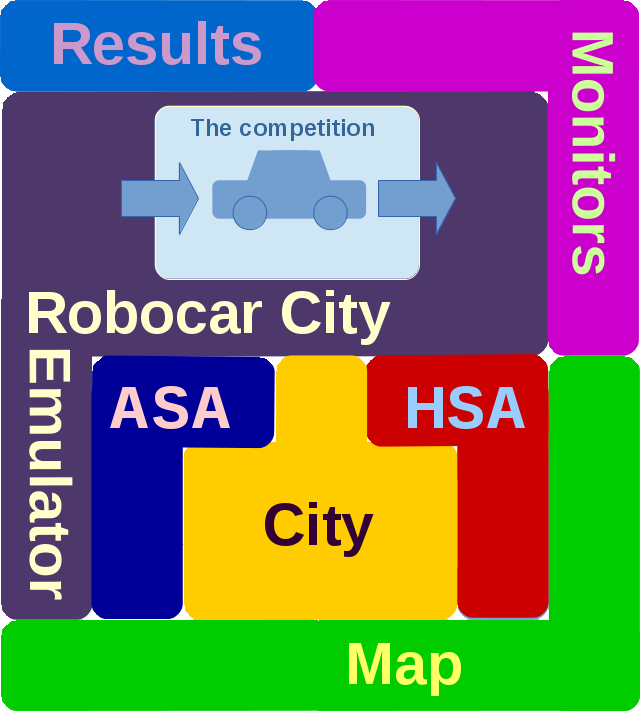
\includegraphics[width=3.4in]{img/tetris_plan}}
\caption{Az OOCWC rendszer tetris terve. Forrás: \cite{oocwcrepo}.}
\label{basedesign}
\end{figure}

Ez alapján a rendszer egyes elemei:

\begin{itemize}
\item Map -- a szimuláció egy adott térképen értelmezett,
\item City -- a szimuláció működési egysége (City Operating Area),
\item The competition -- a verseny célja, illetve maga a verseny,
\item ASA -- automatikus adatgyűjtő rendszer (crowd-sensing),
\item HSA -- kézi adatgyűjtő rendszer (crowd-sourcing),
\item Robocar City Emulator -- forgalom emuláció,
\item Results -- a verseny eredményei, illetve kísérletek eredményei,
\item Monitors -- megjelenítők, vizualizáció.
\end{itemize}

A rendszer többcélú. Egyrészt egy kutatási platformot kínál forgalomelemzésre, szimulációkra. A szimuláció az OpenStreetMap \cite{osm} térképein fut, típusát tekintve a Nagel-Schreckenberg modell \cite{nasch} egy változatának tekinthető, egy cella-alapú megoldás. A rendszer egyik alapkövetelménye, hogy nagyszámú forgalmi egység is reprezentálható legyen. Hasonló esetet mutat be a \cite{singapore} tanulmány, ahol $10^6$ darab járművet szimuláltak. Fontos megjegyezni, hogy ebben a tanulmányban leírt szimuláció nem realisztikus, mivel az egyes egységek nem önálló ágensek. Realisztikus szimulációra is találhatunk példát, \cite{realsim}.

A rendszer másik célja, hogy egy verseny segítségével találjuk meg a lehető legjobb forgalomirányító algoritmust. A rendszer készítő már több sikeres versenyt is lebonyolítottak a Debreceni Egyetem Informatikai Karán \cite{competitions}. Nem ritka, hogy egy-egy kutatási platform versenyezteti a felhasználókat. Erre talán az egyik legjobb példa a mesterséges intelligencia területén a RoboCup \cite{robocup}. 

A rendszer kutatói-fejlesztői folyamata az agilis metodikát követi, gyors prototípusfejlesztéssel az egyes komponensekre. Jelenleg az emulátort tekintve két implementáció létezik, egyrészt a ``Justine'' \cite{oocwcrepo} , másrészt a ``Justina'' \cite{justinarepo}. Mindkét megvalósítás nyílt forráskódú. A rendszerről további információk olvashatóak a \cite{7231223}, valamint \cite{infocomjournal} közleményekben, a ``Justina'' részletes implementációja pedig a \cite{mamenyak2015robotauto} szakdolgozatban.

Kiemelendő, hogy a rendszer magas fokú alkalmazkodóképességgel rendelkezik. Más és más jellegű útvonaltervezés szükséges kormányzati közlekedéshez, vészhelyzetek esetében, stb. Az oktatási és kutatási oldal támogatására került kifejlesztésre a ``Police Edition'' (egy-egy pillanatkép ebből a változatból a \ref{police} ábrán látható). A cél, hogy rendőr ágensekkel, melyeket a kutató által implementált irányító algoritmus vezérel, minél több gengszter ágenst kapjunk el. Egy ilyen implementációra láthatunk példát a \cite{forkcoginfocom} absztraktban.

Az OOCWC rendszerben a szimulációt a gyűjtött adatok alapján inicializáljuk. A rendszer jelenleg háromféle forgalmi egységet különböztet meg, routine cars, smart cars és guided cars. A szimuláció kezdőállapota a routine cars és smart cars elhelyezése a térképen a gyűjtött adatok alapján. (Lásd később részletesen.)

\begin{figure}[h]
\centering
\subfigure{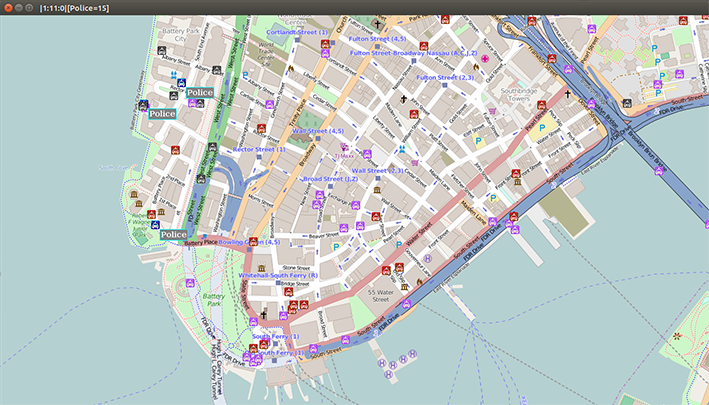
\includegraphics[width=5.3in]{img/m3}\label{p1}}
\quad
\subfigure{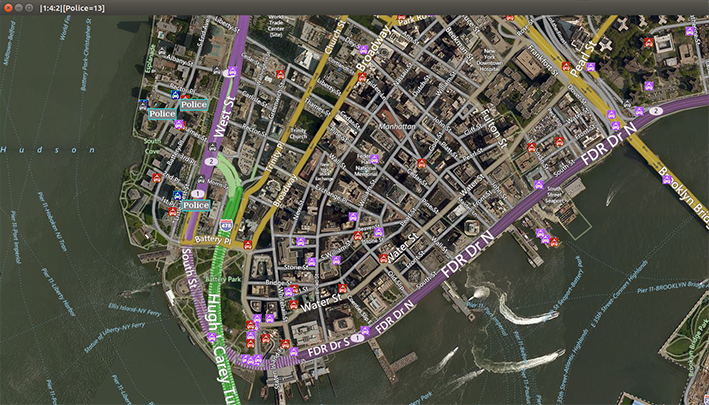
\includegraphics[width=5.3in]{img/m4}\label{p2}}
\caption{Pillanatkép a rendszer ``Police Edition'' változatából. A térkép a OSM egy részlete, Manhattan, New York City, USA. A megjelenítést a JXMapViewer2 \cite{jxmapv} biztosítja. A térképen a routine car rózsaszínnel, a gengszter ágensek pirossal (smart car), a rendőrágensek (guided car) kékkel jelölve. Forrás: \cite{infocomjournal} \label{police}}
\end{figure}

\chapter{Real-time Traffic Analyzer}
\label{rttachapter}

Az adatgyűjtő rendszer hardware és software komponensekből épül fel. A rendszer a Real-time Traffic Analyzer (RTTA) nevet viseli, nyílt forráskódú (GNU GPL v3) és elérhető a projekt tárolójából \cite{rtta}. Megjegyezzük, hogy ez csupán maga az adgyűjtő rendszer. A kimeneti adatokat aggregáció után az OOCWC rendszerben teszteltük. Ehhez szükséges volt annak módosítása, hogy fogadni tudja az adatainkat, így egy fork implementációt készítettünk. Az adatgyűjtő rendszerrel együtt ez a projekt Crowd-sourced Traffic Simulator (CSTS) néven elérhető a GitHubon \cite{csts}. 

Ebben a fejezetben részletesen leírjuk a tervezés lépéseit, milyen szempontok szerint képzeltük a rendszer működését. Ezután részletesen kitérünk az egyes alkotóelemekre, majd a következő fejezetben a CSTS működésére. Ezt követően leírjuk az implementáció során használt fejlesztőeszközöket, majd a tesztelési fázis leírása következik.

\section{Tervezés}
\label{tervezes}

A Robocar City Emulator (RCE) bemeneteként szolgáló adatokat a Robocar City Cloud fogja tárolni. (Jelenleg még nincs ilyen felhőimplementációnk.) Ez az adatbázis fogja tárolni annak a városnak az adatait, ahol az RCE működik. Ahogyan azt már korábban említettük, kétféle adatgyűjtő rendszer-megközelítés létezik. Egyrészt egy közösségi adatgyűjtés, ahol az adatgyűjtők aktív részvétele szükséges egy-egy folyamat megfigyeléséhez és annotálásához. Az OOCWC rendszer sémájában ez a Human controlled Sensor Annotations (HSA) modulnak felel meg. Itt elsősorban olyan mobiltelefonos alkalmazások fogunk kifejleszteni, amely egyszerű grafikus felülettel rendelkezik. Egy használati mód, hogy a megfigyelő egy útszakaszon elhaladó járműveket a mobiltelefon egy softkey-ének a lenyomásával annotálja. A rendszer fejlesztésének jelenlegi fázisában ez a típusú adatgyűjtés még nem implementált.

A másik adatgyűjtő mód az automatikus adatgyűjtés vagy crowd-sensing. Ez a rendszer sémájában a Automatic Sensor Annotations (ASA) modulnak felel meg. Az általunk fejlesztett hardware eszközök felhasználói beavatkozás nélkül képesek adatgyűjtésre. A tervezés első lépéseként meghatároztuk a rendszerrel szemben támasztott alapvető követelményeket. Az alábbiakban összegezhetjük:

\begin{itemize}
\item Valós idejű működés, amely azonnali, lokális képfeldolgozást is lehetővé tesz,
\item Valós idejű, folyamatos adatkapcsolat egy felhő alapú adatbázis megoldással,
\item Pontos helymeghatározás,
\item Egyszerűen beszerelhető járművekbe.
\end{itemize}

A fejlesztést három irányban képzeltük el. A fő különbséget a hardware-ben található processzor (vagy annak hiánya) jelenti. Ami az egyes megoldásokban közös, hogy mindegyikben megtalálható egy FPGA (Field Programmable Gate Array), valamint az egyes perifériák. Bementként egy képszenzort és a GPS vételére alkalmas modult használtunk, kimenetként egy szabványos GSM modult alkalmaztunk. A fejlesztés ún. development boardokon lehetséges. Az egyes hardware designokat az alábbiakban részletezzük.

{\bf{ARM alapú megoldás.}} Ennél a típusnál az FPGA gyorsaságát az I/O rendszer valamint a memória kezelésére használjuk fel. Az ARM processzor egy szabványos opciót kínál számunkra számításokhoz, képfeldolgozó algoritmusok futtatásához. A rendszer fő előnye, hogy könnyedén használhatunk egy Beágyazott Linux Rendszert (Embedded Linux System -- ELS), tehát a magas szintű feldolgozási folyamatokat egy szabványos Linux/UNIX környezetben implementálhatjuk. Ilyen ARM alapú, beágyazott rendszerrel szállított eszköz például a Raspberry Pi single-board számítogép.

{\bf{Soft-processor alapú megoldás.}} Ennél a típusnál nincs fizikailag jelen a processzor, nekünk kell a hardware designhoz hozzáadnunk egy előre definiáltat. (Például a Xilinx Micro-Blaze processzort.) Ebben az esetben mi definiáljuk a processzor pontos működését, de az utasításkészlete limitáló tényező. ELS alkalmazására -- hasonlóan az ARM alapú megoldáshoz -- itt is van lehetőségünk.

{\bf{Nyers FPGA design.}} Ebben az esetben semmilyen processzor nem áll a rendelkezésünkre, csupán az FPGA. Az I/O kezeléstől kezdve a képfeldolgozó algoritmusok futtatásán át a memóriakezelésig minden az FPGA-ban implementált, gyakorlatilag egy tisztán hardware megoldás. Belátható, hogy számítási kapacitás terén ez a leggyorsabb megoldás, ugyanakkor a fejlesztői folyamata is ennek a leghosszabb.

Összegezve a fentieket elmondhatjuk, hogy az ARM alapú megoldások rugalmasabbak, valamint könnyedén bővíthetőek új funkciókkal, de limitálva vagyunk az ARM képességeire (akár az órajelet, akár az utasításkészletet tekintjük).  Ezzel szemben, mivel könnyen és olcsón elérhetőek ilyen fejlesztői kártyák, valamint a fejlesztési folyamat rövidebb és egyszerűbb, hamarabb építhető ki egy fejlesztői közösség a rendszer körül. Az tisztán FPGA alapú designok sokkal gyorsabb feldolgozást tesznek lehetővé, viszont a fejlesztési folyamatuk hosszasabb és komplikáltabb. Jelenleg implementációban az ARM alapú megoldás érhető el, melynek működését ebben a fejezetben részletesen kifejtjük.

\section{Technológiai áttekintés}

Az adatgyűjtő rendszert első körben egy ARM alapú hardware-eszközre fejlesztettük ki. A projekt megvalósításához szükségünk volt egy olyan eszközre, amely sokkal rugalmasabb fejlesztést tesz lehetővé. Ezért például a Raspberry Pi single-board számítógép a szűkös előforrásai, valamint limitált periferizálhatósága miatt nem volt alkalmas a számunkra. (Megjegyezzük, hogy ez csak az eszköz első generációjára érvényes, a második generációs Rapsberry Pi 2 már elfogadható lenne, de az csak a fejlesztés után kerül piacra.) Mivel az ARM egy igen elterjedt processzorcsalád, ezért könnyen elérhetőek fordítóprogramok, illetve egy Beágyazott Linux Rendszer használata is egyszerű. A fent említettek miatt a választásunk egy Zynq System-on-chip (SoC) rendszerre esett.

Ebben a fejezetben részletesen leírjuk a rendszer hardware- illetve software-komponenseit valamint azok működését.

\subsection{Hardware}
\label{rttahw}

A rendszer sémája a \ref{rttaschema} ábrán, a részletes felépítése pedig a \ref{detailedscheme} ábrán látható.

\begin{figure}[h]
\centerline{
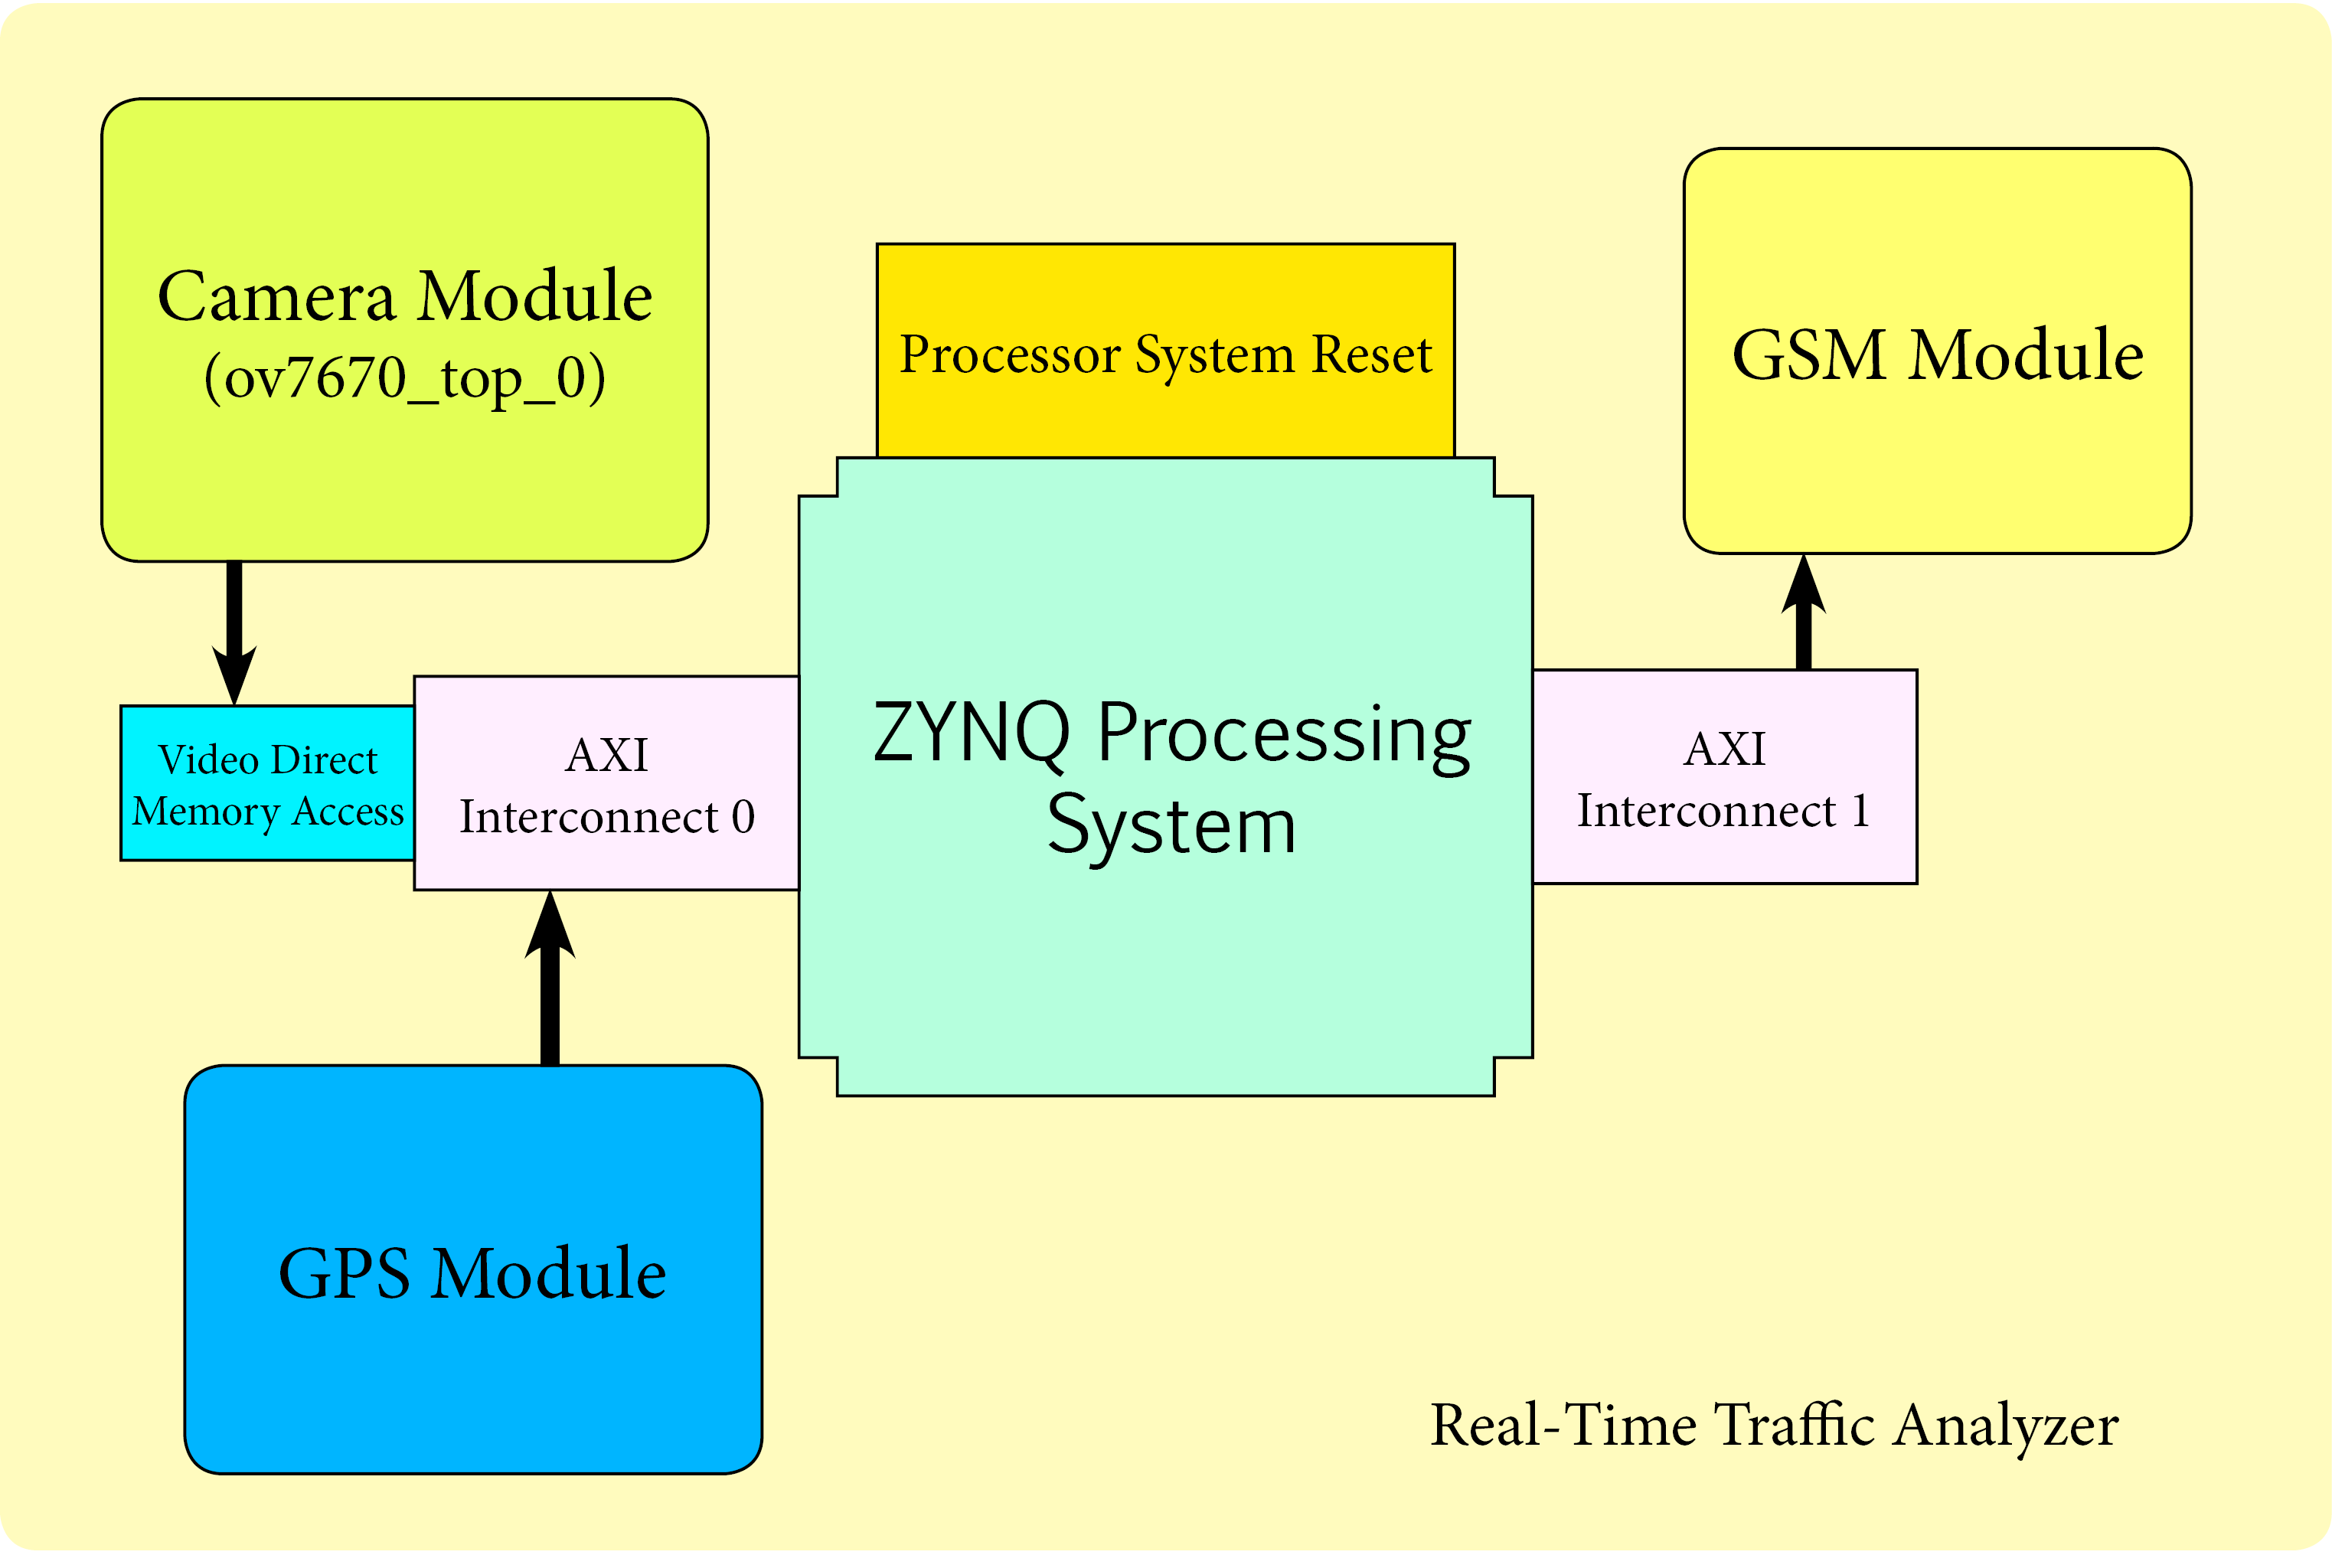
\includegraphics[width=6in]{img/sema}}
\caption{Az RTTA sematikus felépítése. Forrás: \cite{usingcoginfocom}.}
\label{rttaschema}
\end{figure}  

A fejlesztést a Digilent Zybo development boardján végeztük \cite{zybo}. Ahogyan az a sematikus ábrán is látható, a rendszer központi eleme a Zynq Processing System, kiegészülve a Processor System Resettel. Az egyes eszközöket az Advanced Extensible Interface (röveden AXI, \cite{xilinx1999reference}) busz protokollon keresztül kapcsoltuk egymáshoz. Ez a protokoll egy szabványosított megoldást biztosít az egyes komponensek egymáshoz kapcsolására. A két fő komponens a két UartLite soros port. A GPS modullal az \texttt{axi\_uartlite\_0} soros porton kommunikálhatunk, mely 4800 bauddal küldi a GPS 1 PPS adatait. (A GPS 1 másodpercenként küldi a kódméréshez szükséges adatcsomagokat.) A GSM modullal az \texttt{axi\_uartlite\_1} soros porton kommunikálhatunk 115200 bauddal. Az \texttt{ov7670\_top\_0} modul kiolvassa a kamerából a videóadatokat, majd AXI kompatibilis streammé alakítja. Az \texttt{axi\_vdma\_0} betölti a memóriába a kamerából érkező adatokat az \texttt{axi\_interconnect\_0} modulon keresztül.

A kommunikáció az egyes perifériák között az AXI buszon történik. Ennek a busznak 100 MHz-es alapórajele van, a kamera adatok továbbításáért 150 MHz-es másodlagos órajelet alkalmazunk.

Video Direct Memory Access-t (VDMA) alkalmazunk, amely a memória és a kameramodul között közvetlen, nagy sebességű elérést biztosít. Ezzel töltjük be a memóriába a videostreamet. A videó felbontása 640$\times$480 pixel. A VDMA könnyedén használható, és köszönhetően a Linux illesztőprogramnak, könnyedén beintegrálhattuk a rendszerbe.

A céljaiknak a Vincotech A1080-A GPS vevő modulja alkalmasnak tűnik. Minimális külső kompenenseket igényel és egyszerűen soros porton kommunikál. A modul 1 PPS időközönként küld adatot. Ezeket az adatokat a Linux rendszeren futó alkalmazásunk dolgozza fel (lásd a következő fejezetet). A pontos idő és a pozíció fontos a számunkra. A Peripheral Module (PMOD) által leadott áram elegendő ennek a modulnak.

A mobilinternet (GPRS) eléréséhez egy SIM900 GSM modult használtunk. Mivel ez a modul 5V feszültséget igényel, a Zybo belső áramforrására kapcsoltuk. Mivel ilyen kapcsolás esetén a kezdeti áramfelvétel (az ún. initial peak) problémákat tud okozni, ezért erre a jövőben kiemelt figyelmet kell fordítani. Szerencsére a vezeték jelen esetben elbírta a modult, de problémák léphetnek fel, ha egy jármű áramforrásáról próbáljuk az eszközt táplálni.

Képrögzítéshez szerettünk volna egy könnyen paraméterezhető eszközt használni, például egy webkamera helyett. Így esett a választásunk az OV7670-es modulra, könnyen beszerezhető, illetve maximális felbontása (640$\times$480 pixel) elegendő a számunkra. Előnye, hogy paraméterezhető a működése, így pontosan beállíthatjuk a mi igényeinknek megfelelően, illetve a rendszerbe illeszthetősége egyszerűbb. Ennek következménye, hogy a videostream előfeldolgozása nem veszi igénybe a processzort, így az kevésbé válik leterheltté. Jelenleg még nincs hardware szinten előfeldolgozás a rendszerben, de tervezzük egy HLS alapú OpenCV megoldás beépítését.

Fontos kiemelnünk, hogy a jövőben egy CAN buszt is beépítünk a hardware design-ba, így ez az eszköz fog kommunikálni az autóval. Ennek jelentőségére a későbbi fejezetekben térünk ki.

A rendszer jelenlegi állapota a \ref{currentsys} képen látható.

\begin{figure}[h]
\centerline{
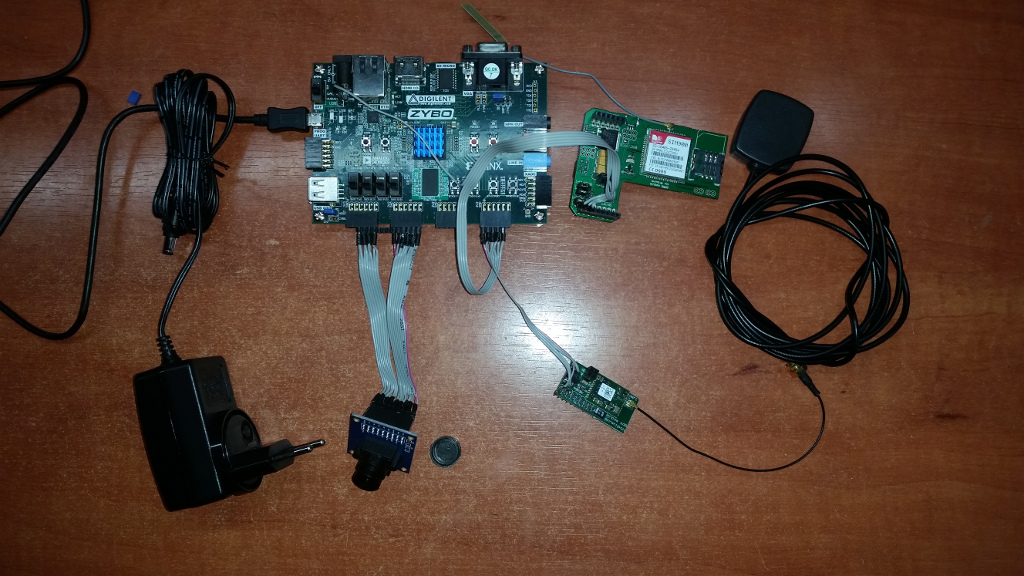
\includegraphics[width=6in]{img/currentsys}}
\caption{A rendszer jelenlegi állapota.}
\label{currentsys}
\end{figure}

Itt jegyezzük meg, hogy a rendszer még nem építhető be civil használatra járművekbe. A tervezés során kiemelt figyelmet kell fordítanunk a járműbe építésre, gyakorlatilag a jármű típusa fogja meghatározni az áramforrás, a befoglaló tartó, illetve egyéb érintésvédelmi szempontok kidolgozását. (Természetszerűleg nem használhatjuk ugyanazt az eszközt buszokban, mint személygépjárművekben.) A fejlesztés jelen fázisában (2015. november) csak belső használatra, illetve a fejlesztők általi tesztelésre alkalmas az eszköz.

\subsection{Software}
\label{rttasw}

Ahogyan azt korábban említettük, az ARM alapú fejlesztői kártyán lehetőségünk van Linux rendszert futtatni. Mi a Linaro mellett döntöttünk, amely egy nyílt forráskódú, Ubuntu Linux alapú, kifejezetten ARM SoC rendszerekre tervezett operációs rendszer. 

Az ezen futó software három részből épül fel.

\begin{itemize}
\item GPS modul,
\item képfeldolgozó modul,
\item GSM modul.
\end{itemize}

A program inicializálja az egyes modulokat, majd minden egyes modult külön szálon elindítja. Ez látható a \ref{main} kódrészletben.

\lstinputlisting[language=C++, caption=A program működése, label=main]{src/main.c}

A GPS modul egyszerűen kiolvassa az eszközről érkező, számunkra lényeges adatokat, majd egy struktúrában eltárolja. Ez látható a \ref{gpsstruct} kódrészletben.

\lstinputlisting[language=C++, caption=A GPS adatstruktúra a számunkra lényeges adatokkal, label=gpsstruct]{src/gpsstruct.cpp}

Kommunikációs protokollnak az MQTT-t választottuk. Az MQTT egy kifejezetten a \texttt{machine-to-machine} típusú kommunikációra kifejlesztett, alacsony overhead-del bíró protokoll. Alapjaiban egy publish/subscribe paradigmát követő megoldás. Kifejezetten jó alacsony fogyasztású eszközök, illetve kis kommunikációs sávszélesség esetén \cite{mqtt}. 

A képfeldolgozó algoritmus egy Haar-cascade osztályozáson alapú objektumfelismerés \cite{violacascade} \cite{haaremp}. Az osztályozás alapjául szolgáló betanított cascade file forrása: \cite{cascade}. A videóstream inicializálása után, minden egyes képet egy Mat típusú objektumban tárolunk, majd a \ref{detectimage} kódrészlettel objektumokat keresünk. 

\lstinputlisting[language=C++, caption=Objektumdetektálás OpenCV-ben, label=detectimage]{src/detectimg.cpp}

Látható, hogy az eszköz nem a nyers képi adatot küldi a szerverünknek, hanem előfeldolgozást végez. A küldött adat formátumát a Google Protocol Buffers segítségével készítettük el. Az üzenet formátuma a \ref{protoobject} kódrészletben látható. 

\lstinputlisting[language=C, caption=Protocol Buffers üzenetformátum, label=protoobject]{src/TrafficAnalytics.proto}

A rendszerhez a tesztelhetőség érdekében készítettünk egy asztali PC-n futtatható alkalmazást. A program egy MQTT szerver alkalmazás, amihez az egyes adatgyűjtő eszközök kapcsolódnak, ide küldik az általuk gyűjtött adatokat. A program bemenete tehát az eszközökről érkező adatok, kimenete pedig egy egyszerű szöveges file, amely az OOCWC rendszer bemeneteként szolgál. Erről részletesebben a következő fejezetben beszélünk.

\section{Fejlesztőeszközök}
\label{dev}

Amint az látható, a rendszer heterogén a felépítését tekinte, ezért több fejlesztőeszköz is szükséges. A hardware design fejlesztését a Xilinx Vivado Design Suite 2014.4-es verziójával végeztük. Az általunk korábban használt fejlesztői eszközhöz képest (Xilinx ISE Design Suite) sok változáshoz kellett alkalmazkodnunk. Míg az ISE alacsony szintű tervezést és implementációt követel meg -- tehát a konkrét Verilog vagy VHDL modul programozását -- addig a Vivado más szempontú fejlesztést tesz lehetővé (természetesen emellett megmaradt a modul programozásának lehetősége is). Ebben a fejlesztői környezetben az egyes kész modulok rendszerbe illesztését egy egyszerűbb, átláthatóbb grafikus felületen tudjuk elvégezni. A mi implementációnk is hasonlóan készült. Első lépésként definiálnunk kell, hogy egy ELS rendszert szeretnénk Zybo development boardon készíteni, majd az egyes perifériákat kell felfűzni a rendszerhez. Fontos megjegyeznünk, hogy nem minden esetben áll rendelkezésünkre előre leírt modul, nekünk a GPS modul működését kellett alacsony szinten definiálnunk.

Az eszközön futó operációs rendszer egyszerűen beépíthető volt a rendszerünkbe, csupán pár apró módosítást kellett elvégeznünk. Ilyen típusú rendszereknél a Linux kernelhez szükséges hozzáadnunk egy általunk definiált ún. device tree-t. Ez a device tree határozza meg, hogy a beágyazott rendszert futtató hardware eszközön az egyes kivezetések (I/O portok) hol helyezkednek el, hol érhetőek el. Ha ezt sikeresen elkészítettük, a Linuxon belülről minden perifériát az ilyen rendszereknél szokott módon, file-ként tudjuk kezelni. Számunkra konkrétan ez azt jelenti, hogy például a GPS modultól érkező adatok egy egyszerű file-ból olvasással, a GSM modul féle küldött adatokat pedig egy egyszerű file-ba írással tudjuk elvégezni. Ilyenre láthatunk példát a \ref{fileops} forráskód részletben. Az első blokk megnyitja olvasásra a GPS modulhoz rendelt file-t, a második pedig elkezdi olvasni. A harmadik blokkban a kameramodulhoz tartozó file-t nyitjuk meg.

\lstinputlisting[language=C++, caption=File műveletek a software-ben, label=fileops]{src/fileoperations.cpp}

A Linux rendszeren futó software-ünket hagyományos Linux/UNIX környezetben tudtuk fejleszteni. Ehhez a KDevelop fejlesztői IDE-t használtuk, szabványos C++11 programnyelven, POSIX szálak segítségével. A képfeldolgozó algoritmust először ki szerettük volna próbálni PC-s környezetben. Ennek oka, hogy jelenleg a RTTA eszközön a megjelenítés nincs implementálva, tulajdonképpen a működést nem tudjuk vizuálisan validálni. A PC-s program ugyanazt az objektumfelismerő algoritmust használja Haar-cascade alapú osztályozás segítségével. A program futását a \ref{rttapc} képen láthatjuk. Bal oldalon látható a videófelvétel (amely egy Apple iPhone 5S-sel készült), itt tájékoztató jellegű adatokat is feltüntettünk, úgymint aktuális pozíció, pontos idő, a felvétel időbélyege, valamint az adott utcán számolt járművek száma. A könnyebb értelmezhetőség érdekében készítettünk egy modult, mellyel térképen tudjuk szemléltetni a bejárt útvonal terheltségét. Ez látható a jobb oldali képen. A \ref{carredrect} képen látható, hogy az algoritmus sikeresen felismeri a járművet a felvételen.

\begin{figure}[h]
\centerline{
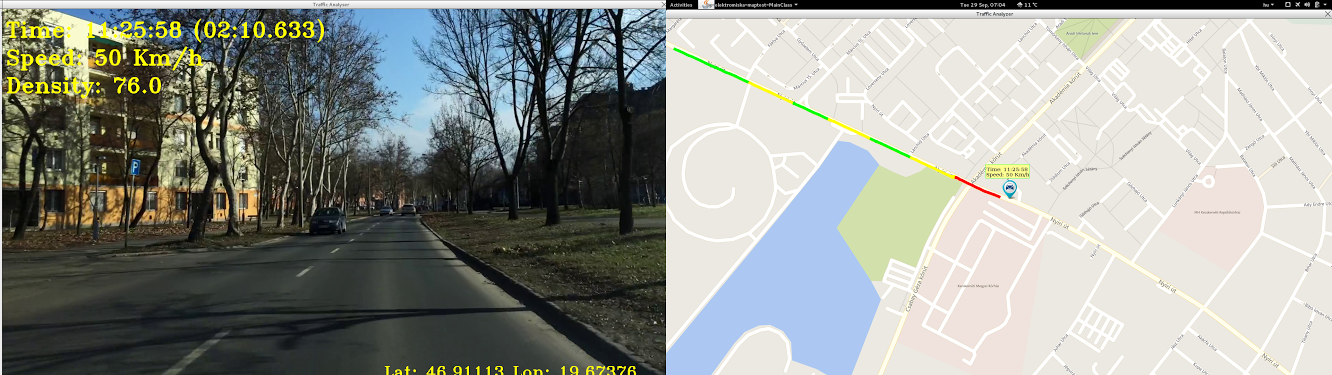
\includegraphics[width=6in]{img/rttapc}}
\caption{A képfeldolgozó algoritmus tesztelése PC-s környezetben.}
\label{rttapc}
\end{figure}

A rendszerhez tartozik egy szerver alkalmazás is, ezt a JAVA 8-as verziójában NetBeans fejlesztői környezetben készítettük. Ez a program fogadja az adatgyűjtő eszköztől érkező adatokat, majd aggregálja azokat. Ennek módszere, hogy a GPS koordináták alapján az osmium fejlesztői könyvtár segítségével minden egyes mért adatot egy utcához rendel, majd a méréseket összegezi. Ez a program állítja elő számunkra azt a file-t, amely a Robocar City Emulator bementeként fog szolgálni (részletesen lásd a következő fejezetben). 

A rendszer felépítéséhez, telepítéséhez nyújt segítséget a projekt hivatalos repozitorijában \cite{rtta} található step-by-step leírás.

\begin{figure}[h]
\centerline{
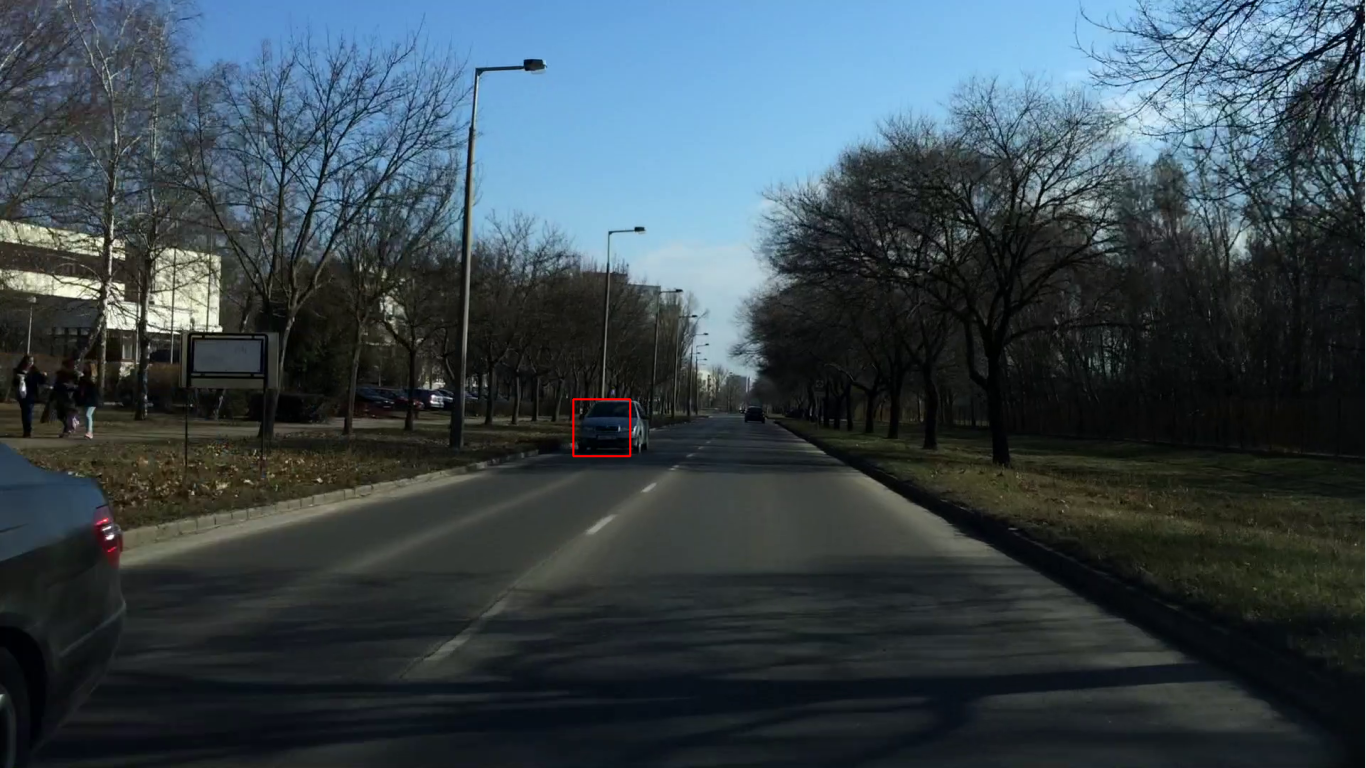
\includegraphics[width=6in]{img/carredrect}}
\caption{Az algoritmus helyes működését szemléltető alkalmazás.}
\label{carredrect}
\end{figure}

\chapter{Crowd-Sourced Traffic Simulator}
\label{cstschapter}

Az RTTA által gyűjtött adatokat az OOCWC rendszer Robocar City Emulator moduljának adtuk meg bemenetként. Ehhez a OOCWC platformból készítettünk egy fork implementációt, majd a mi céljainkra módosítottuk azt. A projektet Crowd-sourced Traffic Simulatornak neveztük el, elérhető a GitHubon \cite{csts}.

A Robocar City Emulator bemente egy szöveges file, mely soronként két információt tartalmaz: az utca nevét és a hozzá tartozó gyakoriságértéket. (Tehát az adott utcán számolt járművek mennyiségét.) A következőkben jelöljük az utcát $s_i$-vel, ($i=1, \dots, N$), a hozzá tartozó gyakoriságértéket pedig $v_i$-vel. Ez a gyakoriság a mérés adott pontjára vagy pontjaira értelmezett az adott utcán. A későbbiekben ez a gyakoriság a pontban mért mérések átlaga lesz. A ``Justine'' szimulátor egy OSM alapú gráfon működik, ahol az egyes csomópontok OSM útpontok. Jelölje $n_i$ a OSM útpont számosságát az $s_i$ utcán és $s_i^j$ a j-edik OSM csomópontot az $s_i$ utcán ($i=1, \dots, N$, $j=1, \dots, n_i$). Ekkor a szimulációban a járművet az $s_i^j$ csomópontra az alábbi valószínűség szerint inicializáljuk: 

\[P(s_i^j)=\frac{v_i}{\sum_{k=1}^{N}{n_kv_k}}.\]

Könnyen belátható, hogy $\sum_{i=1}^{N}\sum_{j=1}^{n_i}P(s_i^j) = 1$.

Tehát a járműveket a szimuláció kezdőállapotában a mért adatok alapján inicializáljuk. Innen indíthatjuk a szimulációt és megfigyelhetjük a szimulációs algoritmus működését.

Az alap OOCWC rendszert szükséges volt egy új osztállyal bővítenünk. Ebben az osztályban reprezentáljuk a valós adatokon alapuló forgalmat. Az új osztály az alap Traffic osztály kiterjesztése (az ősosztály működését lásd az OOCWC projekt dokumentációjában \cite{oocwcrepo}), új tagjai többek között a mért eloszlás adatai, valamint a fent leírt inicializáló módszer alapján egy függvény. Az osztályból a \ref{trafobj}. forráskódrészletben látható módon készítünk egy példányt, amennyiben a célunk a valós adatokon alapuló szimuláció futtatása. Látható, hogy az osztály konstruktorában az \texttt{itype} változóval jelezzük, hogy valós adatok alapján kívánjuk elhelyezni a forgalomban részt vevő járműveket a térképen.

\lstinputlisting[language=C++, caption=A RealTraffic objektum példányosítása, label=trafobj]{src/trafficobj.cpp}

A \ref{nodesel}. forráskódrészletben látható az egyes járművek elhelyezésének módszere. A függvény visszatérési értéke annak -- a térképen található -- csomópontnak az azonosítója (Way Node ID), ahova a járművet a képlet alapján elhelyezzük. A függvény első lépésben összegezi a Way Node ID-ket (8. sor), majd egy véletlen számot generál (11. sor). Ennek a véletlen számnak a segítségével dönt az algoritmus, hogy felteszi-e a járművet az adott node-ra vagy sem.

\lstinputlisting[language=C++, caption=Az inicializálás működése, label=nodesel]{src/nodeselect.cpp}

A mért adatok alapján inicializált szimuláció kezdőállapotát a \ref{simulinit} ábrán láthatjuk. 

\begin{figure}[h]
\centerline{
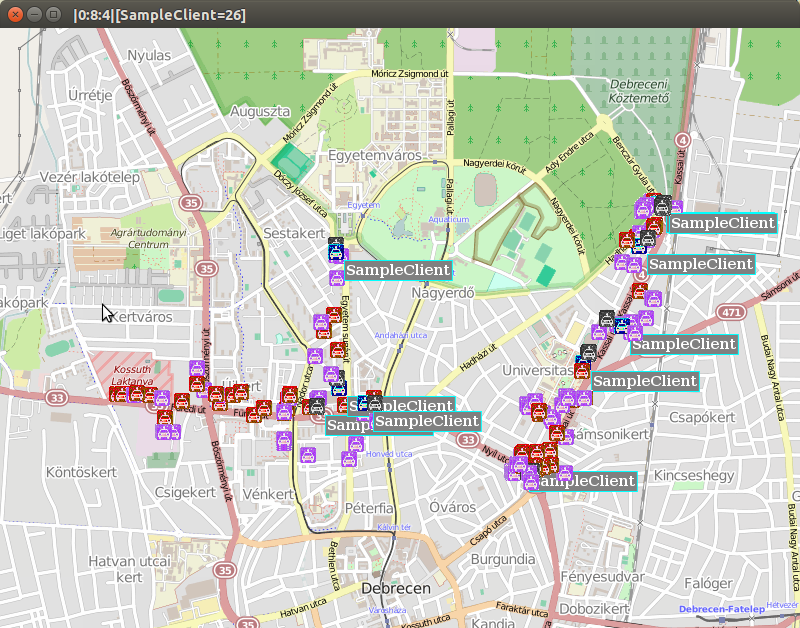
\includegraphics[width=6in]{img/ut3}}
\caption{A mért adatok alapján inicializált szimuláció kezdőállapota. A bementi file az alábbi három sort tartalmazta: Kassai \'ut 789 \textbackslash  Egyetem sug\'ar\'ut 317  \textbackslash  F\"uredi \'ut 559.}
\label{simulinit}
\end{figure}

\chapter{Eredmények}
\label{results}

\section{Adatgyűjtés}

Látható, hogy az OOCWC rendszer fontos építőeleme az adatgyűjtő rendszer. Ahhoz, hogy valós eseményeket szimuláljunk (például útvonaltervezés, valós forgalomszimulációk) a valós világból vett adatokra van szükségünk. Ezt a célt szem előtt tartva, kifejlesztettünk egy tömegérzékelés elven működő rendszert. Az eszköz ARM alapú hardware és software együttese, amely a közeljövőben alkalmas lesz arra, hogy beépítsük forgalomban részt vevő járművekbe. Megjegyezzük, hogy egy kezdetleges tesztelést már végeztünk. Ebben a kísérletben Debrecen néhány utcáját vizsgáltuk és az így kapott adatokat a Robocar City Emulator bemeneteként használtuk. Az adatgyűjtő rendszer neve Real-time Traffic Analyzer, az erre, valamint az OOCWC rendszerre épülő projekt neve Crowd-sourced Traffic Simulator.

A kifejlesztett adatgyűjtő eszköz, amelyet folyamatosan mozgó járművekbe fogunk telepíteni képes forgalmat mérni, konkrétan a környezetében kialakult forgalmi helyzetet. Fontos megjegyezni, hogy a rendszer újszerűségét az adja, hogy az eszköz folyamatosan mozgásban van. Több, hasonló célra fejlesztett adatgyűjtő rendszer üzemel, de azok mind fix telepítésűek. Emiatt minden egyes speciális tényezőt figyelembe kellett vennünk a tervezés során. Az eszköz központi eleme egy fejlesztői kártya, amely jelenleg egy Digilent Zybo. Ez a kártya egy FPGA-t és egy ARM processzor tartalmaz, melyek egymást kiegészítve működnek. Az FPGA végzi az I/O rendszer kezelését, az ARM processzor a képfeldolgozást végzi. Mivel az eszköz folyamatosan mozgásban van, szükséges volt egy GPS modul is, így meghatározhatjuk az eszköz pontos helyét, valamint az egyes gyakoriságértékeket utcákhoz rendelhetjük. Maga a képfeldolgozás egy Haar-cascade alapú osztályozás, és egy erre épülő objektumfelismerés. A videostream-et egy kameramodultól kapjuk 640$\times$480 pixel felbontásban. Az adatokat előfeldolgozás után mobilinterneten küldjük a szerveralkalmazásunknak egy szabványos GSM modul segítségével.

A Zybo fejlesztői kártya jelenleg elegendő, de ha bővíteni szeretnénk új funkciókkal, könnyen lehet, hogy kevésnek bizonyul. Problémát okozhat, ha szeretnénk bizonyos képi előfeldolgozást végezni a SoC FPGA részében. A perifériák jól működnek, de valószínűleg a kommunikációs interface-t egy USB-s mobilstickkel fogjuk helyettesíteni.

A mérés egy autószámláló eljárás, amely minden egyes útszakaszon egy sűrűségértéket ad. Minél több járművet számolunk adott útszakaszon, annál sűrűbb ott a forgalom. A szerveroldalon egy algoritmus összegyűjti ezeket a sűrűségadatokat, majd aggregáció után utcákhoz rendeli. Így a program egy file-t állít elő, melyben minden sor két értéket tartalmaz: az utca nevét és az utcához tartozó gyakoriságot.

A szimuláció során ezt a gyakoriságértéket használjuk. A Robocar City Emulator bementén megadjuk ezt az egyszerű szöveges állományt, amely ez alapján inicializálja a szimuláció kezdőállapotát. Ezután a szimulációt elindítjuk, majd megfigyeljük hogyan változik a járművek eloszlása. Az OOCWC rendszert egy flexibilis rendszernek tartják. Ez alatt azt értjük, hogy könnyedén testre szabható (más szempontok szerint kell útvonalat tervezni például kormányzati közlekedésnek, hatósági vagy életmentő beavatkozások során). A CSTS rendszer bizonyítja, hogy a rendszer valóban rugalmas, amely ezzel egy nagy lépést tett a céljai felé. 

Megjegyezzük, hogy az adatgyűjtő rendszer rendben működött a tesztelési fázis során. Az objektumfelismerő algoritmus csaknem minden járművet felismert, pontos pozíciót tudott szolgáltatni, valamint az adatok rendben megérkeztek a szerveralkalmazásunkhoz. A Robocar City Emulator egy kisebb fejlesztés után képes volt szimulálni a valós adatokon alapuló forgalmi viszonyokat. 

\section{Forgalomszimuláció az OOCWC rendszerben}

A CSTS rendszerben a szimuláció kezdeti állapotában a járműveket a mért adatok alapján számolt eloszlás szerint tettük fel a térképre. Ez látható a \ref{simulinit} ábrán. Célunk volt annak megfigyelése, hogyan változik a szimuláció során az autók eloszlása a kezdeti eloszláshoz képest. A \ref{hista}, \ref{histb} és \ref{histc} diagramokon láthatjuk, hogyan változik az eloszlás a szimuláció futásával. (A szimuláció Debrecen város gráffal reprezentált térképén értelmezett.) Az x tengelyen az utcákat, az y tengelyen az azonos utcán található autók számát jelöltük. Csak azok az utcák reprezentáltak a hisztogramon, amelyek legalább egy autót tartalmaznak. A hisztogramok Debrecen utcáit a rajtuk található autók száma szerint rendezve mutatják csökkenő sorrendben. Érdemes megfigyelni, hogy az eloszlás jellege (Pareto) nem változik a szimuláció során, viszont az utcák sorrendje felcserélődik. Természetes, hogy új utcák lépnek be az eloszlásba, viszont fontos kritérium, hogy az utcák sorrendje nem változhat a szimuláció során. (Meg kell követelnünk a szimulációs algoritmustól egyféle stacionaritást.) Jelenleg az OOCWC-ben található szimulációs algoritmus nem teljesíti ezt a feltételt.

\begin{figure}[h]
\centerline{
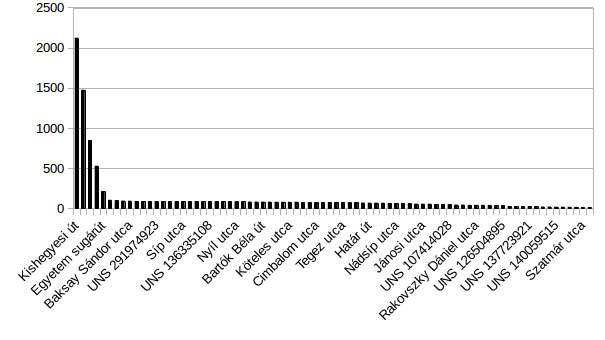
\includegraphics[scale=.8]{img/a1}}
\caption{A szimuláció kezdetekor az uták száma: 78.}
\label{hista}
\end{figure}

\begin{figure}[h]
\centerline{
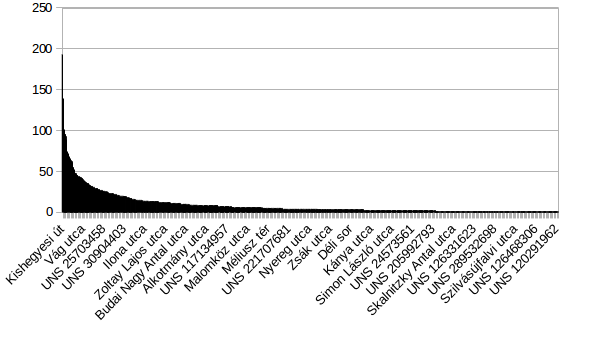
\includegraphics[scale=.8]{img/a2}}
\caption{Egy perc elteltével az uták száma: 1085.}
\label{histb}
\end{figure}

\begin{figure}[h]
\centerline{
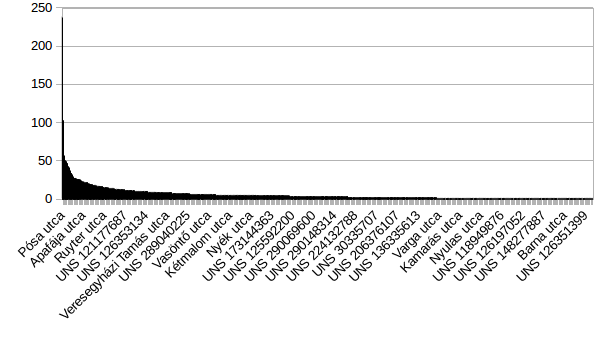
\includegraphics[scale=.8]{img/a3}}
\caption{Tíz perc elteltével az utcák száma: 1725.}
\label{histc}
\end{figure}

A tesztelés során 10000 járművet inicializáltunk a mért adatokon számolt eloszlás alapján. Ez a \ref{simultenth} ábrán látható.

\begin{figure}[h]
\centerline{
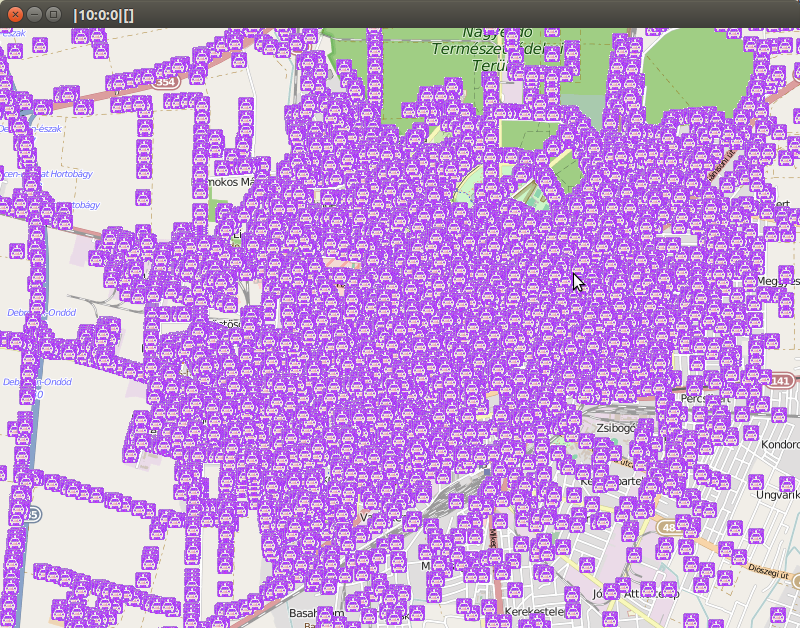
\includegraphics[scale=.5]{img/a33}}
\caption{Pillanatkép a szimulációból.}
\label{simultenth}
\end{figure}

\chapter{Jövőbeli munka}

\todo[inline]{Több eszközös mérés, City Cloud, Szimulációs algoritmus eloszlástartó legyen.}

\chapter{Összefoglalás}

\todo[inline]{Max 2 oldalas összegzés.}

\addcontentsline{toc}{chapter}{Irodalomjegyzék}

\bibliography{rtta}

\chapter*{Egyéb tudnivalók}

A diplomamunka alapjául az alábbi közlemények szolgálnak:

Bátfai, N.; {\bf{Besenczi, R.}}; Mamenyák, A.; Ispány, M., {\bf{"OOCWC: The Robocar World Championship Initiative,"}} in Telecommunications (ConTEL), 2015 13th International Conference on, pp.1-6, 13-15 July 2015, doi: 10.1109/ ConTEL.2015.7231223

N. Bátfai, {\bf{R. Besenczi}}, A. Mamenyák and M. Ispány. {\bf{"Traffic Simulation based on the Robocar World Championship Initiative."}} INFOCOMMUNICATIONS JOURNAL, vol. 7, no. 3, 2015, pp. 50-59.

{\bf{Besenczi R.}}; Katona T.; Szilágyi M., {\bf{"A Fork Implementation of the Police Edition of the OOCWC System,"}} in Cognitive Infocommunications (CogInfoCom), 2015 6th IEEE Conference on, pp.163-164, 19-21 Oct. 2015, doi: Not yet assigned

{\bf{Besenczi R.}}; Szilágyi M.; Bátfai N.; Mamenyák A.; Oniga I.; Ispány M., {\bf{"Using Crowdsensed Information for Traffic Simulation in the Robocar World Championship Framework,"}} in Cognitive Infocommunications (CogInfoCom), 2015 6th IEEE Conference on, pp.333-337, 19-21 Oct. 2015, doi: Not yet assigned

A Real-time Traffic Analyzer projekt nyílt forráskódú (GNU GPL v3), szabadon felhasználható és letölthető a projekt hivatalos tárolójából: \cite{rtta}.

A Crowd-sourced Traffic Simulator projekt nyílt forráskódú (GNU GPL v3), szabadon felhasználható és letölthető a projekt hivatalos tárolójából: \cite{csts}.

A Robocar World Championship hivatalos oldala, illetve a tároló: \cite{oocwcrepo}.

\addcontentsline{toc}{chapter}{Egyéb tudnivalók}

\chapter*{Függelék}
\addcontentsline{toc}{chapter}{Függelék}

\noindent
RTTA is free software: you can redistribute it and/or modify
it under the terms of the GNU General Public License as published by
the Free Software Foundation, either version 3 of the License, or
(at your option) any later version.

\noindent
RTTA is distributed in the hope that it will be useful,
but WITHOUT ANY WARRANTY; without even the implied warranty of
MERCHANTABILITY or FITNESS FOR A PARTICULAR PURPOSE.  See the
GNU General Public License for more details.

\noindent
You should have received a copy of the GNU General Public License
along with RTTA. If not, see <http://www.gnu.org/licenses/>.

\noindent
CSTS is free software: you can redistribute it and/or modify
it under the terms of the GNU General Public License as published by
the Free Software Foundation, either version 3 of the License, or
(at your option) any later version.

\noindent
CSTS is distributed in the hope that it will be useful,
but WITHOUT ANY WARRANTY; without even the implied warranty of
MERCHANTABILITY or FITNESS FOR A PARTICULAR PURPOSE.  See the
GNU General Public License for more details.

\noindent
You should have received a copy of the GNU General Public License
along with CSTS. If not, see <http://www.gnu.org/licenses/>.


\begin{sidewaysfigure}
    \centering
    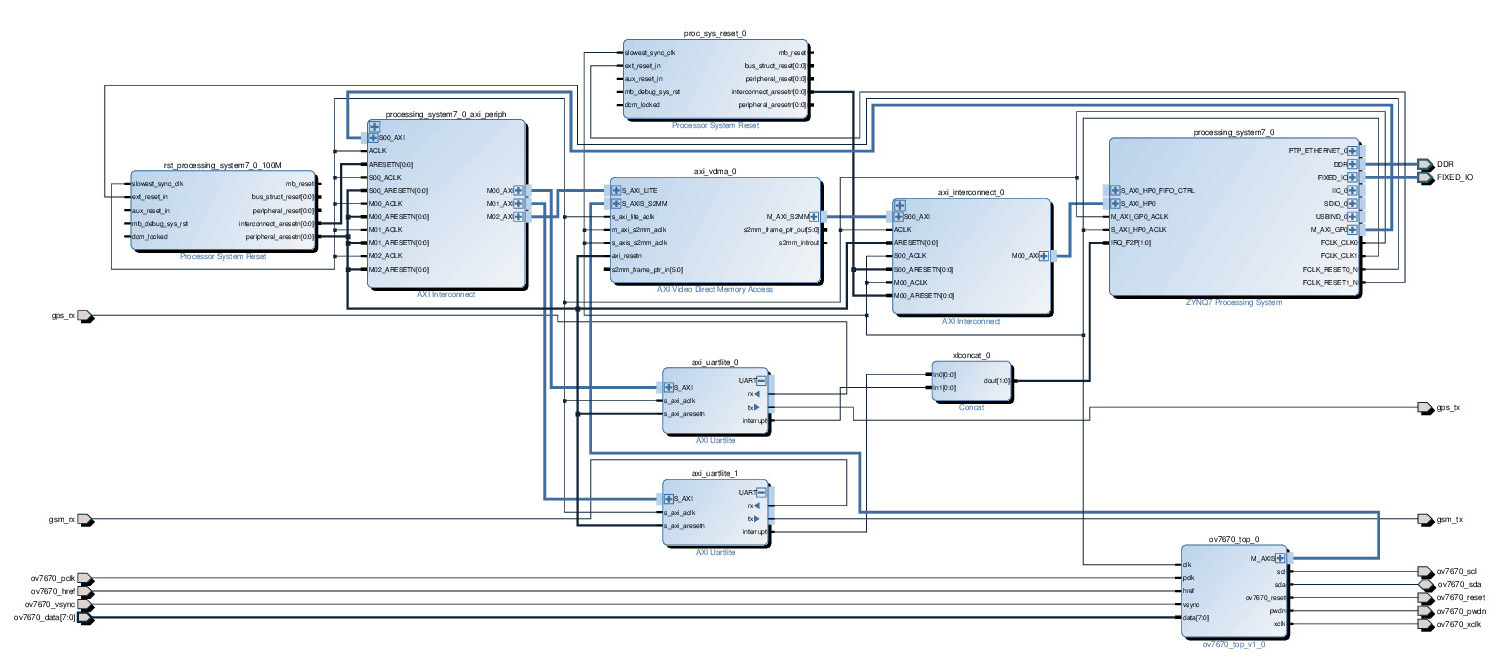
\includegraphics[width=10in]{img/base_design_1}
    \caption{Az RTTA részletes sémája.}
    \label{detailedscheme}
\end{sidewaysfigure}

\chapter*{Köszönetnyilvánítás}
\addcontentsline{toc}{chapter}{Köszönetnyilvánítás}

\end{document}
